\documentclass[12pt]{article}

%% Useful packages
\usepackage[a4paper,top=1.2in,bottom=1.2in,left=1in,right=1in,marginparwidth=1.75cm]{geometry}
\usepackage{amsmath}
\usepackage{amsfonts}
\usepackage{algorithm}
\usepackage{algorithmic}
\usepackage{cite}
\usepackage{courier}
\usepackage{caption}
\usepackage{graphicx}
\usepackage[colorlinks=true, allcolors=red]{hyperref}
\usepackage{float}
\usepackage{setspace}
\usepackage{subfigure}
\usepackage{url}
\usepackage{tabularx}
\usepackage[utf8]{inputenc}
\usepackage{mathptmx} %Times Font

\begin{document}
%==== FRONT PART====
\begin{titlepage}

\begin{figure}[H]
\centering

\includegraphics[width=\textwidth]{Title/logo.png}
\caption*{}\label{fig:entropy} 
\end{figure}

\centering
\LARGE{\textbf{AI6121:}}\\
\LARGE{\textbf{Image Translation and UDA}}\\[2.0in]

\large{\textbf{Rao Yixi, G2302775D}}\\
\large{\textbf{Jin Zhixiao, G}}\\
\large{\textbf{Huang Siwei, G}}\\[1in]

\textbf{School Of Computer Science And Engineering}\\[0.75in]

\textbf{18/11/2023}
\newpage
\end{titlepage}

\pagenumbering{plain}
\tableofcontents

%==== MAIN PART ====
\pagenumbering{arabic}
\section{Introduction}
s

\newpage
\section{Image-to-Image Translation}
\paragraph{}
The image to image translation model we chose is Cycle Generative Adversarial Network (CycleGAN) developed by Zhu et al~\cite{zhu2017unpaired}.

\subsection{Introduction}
\paragraph{}
For image-to-image translation task, an original image set $S$ and a target image set $T$ are required. For most of the current I2I models, the two image sets used for training need to be paired, meaning that for every image $s \in S$, there must be a corresponding image $t \in T$. However, this kind of paired image set is scarce because (1) Manual production is time-consuming and laborious (2) The target image set required by some vision and graphics tasks does not exist, such as image translation between painters of different styles. The CycleGAN model proposed by Zhu et al.\ is designed to solve the unpaired image-to-image translation problem. 

The CycleGAN model needs to learn a mapping $G: S \rightarrow T$ between an input image and an output image, which can take the special features of the original image set, and then figure out how to transform these features to the target image set, making it difficult to distinguish between the translated image distribution and the target image set distribution. However, this kind of unpaired unidirectional I2I translation will have an under-constrained problem, that is, the translated image distribution $G(s)$ does match the target image set, but it cannot correspond to the original image $s$ in a meaningful way. This is because there are many mappings $G$ that can generate images with the same distribution. Moreover, this unidirectional training also triggers the well-known problem of mode collapse.

Zhu et al.\ used the property that translation should be ``cycle consistent'' to define another mapping $F: T \rightarrow S$ to reproject the translated image onto the original image, ensuring that $F(G(s))=s$ and $G(F(t))=t$. The model uses two generators and their corresponding discriminators using adversarial loss and defines a novel cycle consistency loss to train the two generators, and discriminators simultaneously. Figure~\ref{figure:cyclegan} shows the basic design of CycleGAN and the Loss definition.

\begin{figure}[!ht]
    \centering
    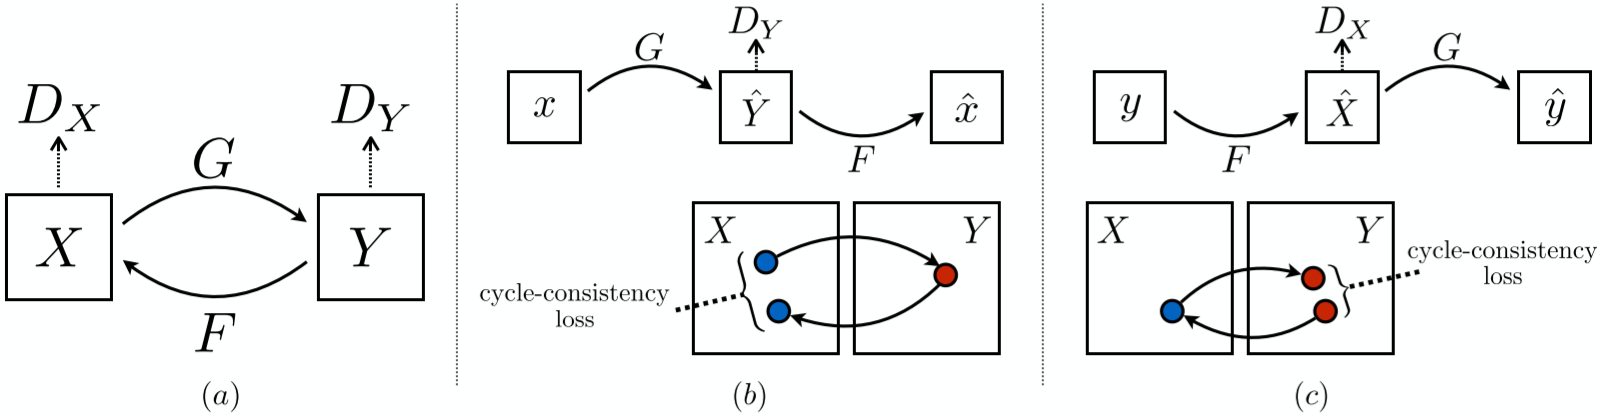
\includegraphics[width=0.9\textwidth]{Section2/cycleGAN.png}
    \caption{(a) The model contains two mapping functions (generators) and associated adversarial discriminators (b) forward cycle-consistency loss (c) backward cycle-consistency loss.}\label{figure:cyclegan}
\end{figure}

\subsection{Model Architecture}
\paragraph{}
To accomplish I2I, the overall model contains two generators $G: S \rightarrow T$ and $F: T \rightarrow S$ and the corresponding two adversarial discriminators $D_S$ and $D_T$, which are used to distinguish between the original image and the translated image. The basic idea is to improve the accuracy of the adversarial discriminators on image sets $S$ or $T$ while improving the image translation ability of the generators. The ideal result is that the discriminators maintain high accuracy on the image sets $S$ or $T$, but only 50\% accuracy in recognizing the fake images translated by the generators.

\paragraph{Adversarial Loss.}Adversarial loss is applied to generators and discriminators and is mainly used to ensure that the levels of sets of translations from domain S (T) and domain T (S)  are appropriate. Below is the adversarial loss for $G$ and $D_T$. The other one is similar.

\begin{equation}
    \mathcal{L}_{GAN}(G,D_T,S,T) = \mathbb{E}_{t \sim p_{data(t)}}[\log D_T(t)] + \mathbb{E}_{s \sim p_{data(s)}}[\log(1 - D_T(G(s)))]
\end{equation}

\paragraph{Cycle Consistency Loss.} 
To ensure cycle consistency, a reproject error-like forward cycle consistency loss and backward cycle consistency loss, corresponding to two generators respectively, are used, which are defined as:

\begin{equation}
    \mathcal{L}_{cyc}(G,F) = \mathbb{E}_{s \sim p_{data(s)}}[||F(G(s)) - s||_{1}] + \mathbb{E}_{t \sim p_{data(t)}}[||G(F(t)) - t||_{1}]
\end{equation}

Therefore, the full objective function can be defined as:

\begin{equation}
    G^*,F^* = \arg \mathop{\min}_{G,F} \mathop{\max}_{D_S,D_T} \mathcal{L}(G,F,D_T,D_S)
\end{equation}

\begin{equation}
    \mathcal{L}(G,F,D_T,D_S) = \mathcal{L}_{GAN}(G,D_T,S,T) + \mathcal{L}_{GAN}(G,D_S,T,S) + \lambda \mathcal{L}_{cyc}(G,F)
\end{equation}

\subsection{Implementation}
\paragraph{}
We have organized the implementation of CycleGAN into four steps. The first step is to define the dataset and pre-processing, the second step is to define the discriminator model, the third step is to define the generator model, and the fourth step is to define the training for CycleGAN.\@ We use Pytorch to implement CycleGAN and refer to the source code of Zhu et al~\cite{zhu2017unpaired} and Aladdin's code reproduction~\cite{CycleGANcode}. Here we only present the core codes, please check the source code for detailed implementation.

\subsubsection{Dataset \& Pre-processing}
\paragraph{}
We use the GTA5 video game street view from~\cite{richter2016playing} as the original dataset $S$ and the real cityscape dataset from~\cite{cordts2016cityscapes} as the $T$ dataset, so our goal is to convert the GTA5 video game street view image into a real street view style image. The image augmentation we use is, to resize the image to 180 $\times$ 360, then use horizontal flip on the image with $p = 0.5$, and finally normalize all the image channels to have a mean of 0.5 and standard deviation of 0.5. Finally, convert it to tensor. The detailed implementation is shown below.

\begin{python}
A.Compose([A.Resize(width=360, height=180),
                    A.HorizontalFlip(p=0.5),
                    A.Normalize(mean=[0.5, 0.5, 0.5],
                                std=[0.5, 0.5, 0.5], 
                                max_pixel_value=255),
                    ToTensorV2()])
\end{python}

\subsubsection{Discriminator Model}
\paragraph{}
The implementation of discriminator architectures follows the paper description of Zhu et al., who use 70 $\times$ 70 PatchGAN as the discriminator model. Define \pyth{Ck} as 4 $\times$ 4 Convolution-InstanceNorm-LeakyReLU layer with k filters and stride 2. We use Pytorch's \pyth{nn.Module} to define \pyth{Ck} block class:

\begin{python}
self.conv = nn.Sequential(
    nn.Conv2d(
        in_channels, 
        out_channels,
        4, 
        stride, 
        1, 
        bias=True,
        padding_mode="reflect"
    ),
    nn.InstanceNorm2d(out_channels),
    nn.LeakyReLU(0.2, inplace=True)
)
\end{python}

We then connect four \pyth{Ck} blocks in the order of C64-C128-C256-C512 as the discriminator architecture, where the C64 block does not use the InstanceNorm layer.\ Finally we use a convolution to produce a 1-dimensional output and add the sigmoid function.

\subsubsection{Generator Model}
\paragraph{}
The Generator architecture used by Zhu et al.\  consists of a convolution block and a residual block, where the convolution block is divided into downsampling and upsampling blocks. In the following, we use \pyth{nn.Module} define convolution block as:

\begin{python}
# Downsampling layers or upsampling layers
self.conv = nn.Sequential(
    nn.Conv2d(in_channels, 
              out_channels, 
              padding_mode="reflect", 
              **kwargs) 
              if down
              else 
              nn.ConvTranspose2d(in_channels,
                                 out_channels, 
                                 **kwargs),
    nn.InstanceNorm2d(out_channels),
    nn.ReLU(inplace=True) if use_act else nn.Identity()
)
\end{python}

Based on this convolution block class, we can define three types of convolution blocks. The first is the \pyth{c7s1-k} block, which uses a 7 $\times$ 7 Convolution-InstanceNorm-ReLU layer with k filters and stride 1. The second is the downsampling block \pyth{dk}, which uses a 3 $\times$ 3 Convolution-InstanceNorm-ReLU layer with k filters and stride 2. The third is the upsampling block \pyth{uk}, which is a 3 $\times$ 3 fractional-strided-Convolution-InstanceNorm-ReLU layer with k filters and stride $\frac{1}{2}$.

For residual block, it is two 3 $\times$ 3 convolutional layers with the same number of filters on both layer. We defined it as the residual block (below) class using \pyth{nn.Module}. The \pyth{forward} function is \pyth{return x + self.block(x)}.

\begin{python}
self.block = nn.Sequential(
    ConvBlock(channels,
              channels, 
              kernel_size=3, 
              padding=1),
    ConvBlock(channels, 
              channels, 
              use_act=False, 
              kernel_size=3, 
              padding=1)
)
\end{python}

We build the generator network as: ``c7s1-64,d128,d256,R256,R256,R256,R256, R256,R256, R256, R256, R256, R256, R256, R256, R256, R256, u128
u64,c7s1-3'', and followed by a tanh activation function.

\begin{python}
# c7s1-64
x = self.initial(x)
# d128,d256
for layer in self.down_blocks:
    x = layer(x)
# R256,R256,R256,R256,R256,R256,R256,R256,R256
x = self.res_blocks(x)
# u128 u64
for layer in self.up_blocks:
    x = layer(x)
# c7s1-3
return torch.tanh(self.last(x))
\end{python}

\subsubsection{Training}
\paragraph{}
When implementing training, we adopted Zhu et al.`s training details and their recommended settings, such as training parameter settings:

\begin{itemize}
    \item Use a batch size of 2 to prevent out of memory.
    \item A total of 200 epochs are trained, of which the learning rate is kept constant for 100 epochs, and the decay learning rate strategy is used for the other 100 epochs. Here we use the cosine annealing learning rate strategy.
    \item Set the initial learning rate to 0.0002
    \item Set cycle consistent control factor $\lambda = 10$
    \item Use Adam solver
\end{itemize}

At the same time, we adopt their recommended improvement techniques, such as using least-squares loss to replace the negative log likelihood objective in $\mathcal{L}_{GAN}$. This loss is more stable during training and generates higher quality results. Therefore, the new goal will be:

\begin{itemize}
    \item When training $G$ or $F$: minimize 
    \[\mathbb{E}_{s \sim p_{data(s)}}[{(D_T(G(s)) - 1)}^2] +\] 
    \[\mathbb{E}_{t \sim p_{data(t)}}[{(D_S(F(t)) - 1)}^2] +\] 
    \[\mathcal{L}_{cyc}(G,F)\]
    \item When training $D_S$ or $D_T$: minimise 
    \[\mathbb{E}_{s \sim p_{data(s)}}[{(D_S(s) - 1)}^2] + \mathbb{E}_{t \sim p_{data(t)}}[{D_S(F(t))}^2] +\] 
    \[\mathbb{E}_{t \sim p_{data(t)}}[{(D_T(t) - 1)}^2] + \mathbb{E}_{s \sim p_{data(s)}}[{D_T(G(s))}^2]\]
\end{itemize}

Following the above training setting, for each batch images (source, target), we first train the discriminators $D_T$ and $D_S$. We can obtain two discriminators' result by using corresponding generators.

\begin{python}
# Patch: DT(T) and DT(GT(S))
DT_real = disc_T(target)
DT_fake = disc_T(gen_T(source))

# Patch: DS(S) and DS(GS(T))
DS_real = disc_S(source)
DS_fake = disc_S(gen_S(target))
\end{python}

And then we can calculate the $\mathcal{L}_{GAN}$ losses with respect to discriminators $D_T$ and $D_S$.

\begin{python}
# L_GAN(GT,DT,S,T) = minimize Et[(DT(t) - 1)^2] + Es[DT(GT(s))^2]
DT_real_loss = mse(DT_real, torch.ones_like(DT_real))
DT_fake_loss = mse(DT_fake, torch.zeros_like(DT_fake))
# L_GAN(GT,DT,S,T)
DT_loss = DT_real_loss + DT_fake_loss

# L_GAN(GS,DS,S,T) = minimize Es[(DS(s) - 1)^2] + Et[DS(GS(t))^2]
DS_real_loss = mse(DS_real, torch.ones_like(DS_real))
DS_fake_loss = mse(DS_fake, torch.zeros_like(DS_fake))
# L_GAN(GS,DS,S,T) 
DS_loss = DS_real_loss + DS_fake_loss
\end{python}

Finally, we put it together to get the total adversarial loss, and then train the model with the defined optimizer to opitmize discriminators.

\begin{python}
# put it togethor: L_GAN(GT,DT,S,T) + L_GAN(GS,DS,S,T) 
D_loss = (DT_loss + DS_loss) / 2
\end{python}

Next, we need to train the generators $G_t$ and $G_S$. In the full objective function, the two generator models appear both in adversarial loss and cycle consistency loss. To compute the adversarial loss in terms of generators, the results of the discriminators are first computed for the forward and backward translated images.

\begin{python}
# Patch: DT(GT(S)) and DS(GS(T)) 
DT_fake = disc_T(gen_T(source))
DS_fake = disc_S(gen_S(target))
\end{python}

Then we need to compute the adversarial loss with respect to generators.

\begin{python}
# minimize Et[(DT(t) - 1)^2] and Es[(DS(s) - 1)^2]
loss_GT = mse(DT_fake, torch.ones_like(DT_fake))
loss_GS = mse(DS_fake, torch.ones_like(DS_fake))
\end{python}

To compute the cycle consistency loss, which only concludes the generators, we first need to get the reprojection of the translated images.

\begin{python}
# GS(GT(S)) -> S'
cycle_source = gen_S(gen_T(source))
# GT(GS(T)) -> T'
cycle_target = gen_T(gen_S(target))
\end{python}

And then calculate the cycle consistency loss according to the definition shown above. Finally, minimising the cycle consistency loss by using the defined optimizer to opitmize the generators model.

\begin{python}
# Lcyc(GS,GT) = Es[|GS(GT(s)) - s|] + Et[|GT(GS(t)) - t|]
cycle_source_loss = l1(source, cycle_source)
cycle_target_loss = l1(target, cycle_target)

# add all togethor: L(GS,GT,DS,DT) = LGAN(GT,DT,X,Y) + LGAN(GS,DS,X,Y) + Lcyc(GS,GT)
G_loss = loss_GT + loss_GS +  
         lambda * (cycle_source_loss + cycle_target_loss) 
\end{python}

\subsection{Result Discussion}

\subsubsection{Result presentation}
\paragraph{}
We randomly sampled 3000 images from GTA5 image set and 3000 images from cityscape image set for training and continued to randomly sample 1000 images from the remaining GTA5 image set for testing. Figure~\ref{figure:cycgantest} are the results of the test which contains the testing results from the training set and the results from the test set. We can observe that our CycleGAN recognizes color and texture variations excellently across different image sets and successfully converts video game cityscapes to real-world style cityscapes. It performs better on the training set than on the test set, which conforms to our expectations. Note that the converted image on the test set seems to be slightly blurry compared to the image on the training set, and there may be some color distortion.

\begin{figure}[!ht]
    \setlength\tabcolsep{6pt}
    \adjustboxset{width=\linewidth, valign=c}
    \centering
    \begin{tabularx}{1.0\linewidth}{@{}
        l @{\hspace{4pt}}
        X @{\hspace{4pt}}
        X @{\hspace{6pt}} |
        X @{\hspace{4pt}}
        X @{\hspace{4pt}}
      @{}}
      & \multicolumn{1}{c}{\footnotesize \textbf{Source:} Train set}
      & \multicolumn{1}{c}{\footnotesize \textbf{Target:} Train set}
      & \multicolumn{1}{c}{\footnotesize \textbf{Source:} Test set}
      & \multicolumn{1}{c}{\footnotesize \textbf{Target:} Test set} \\
      \rotatebox[origin=c]{90}
      & 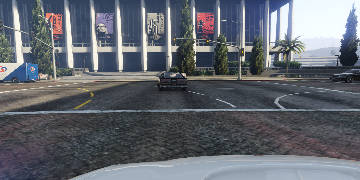
\includegraphics{Section2/train/02003_real.png}
      & 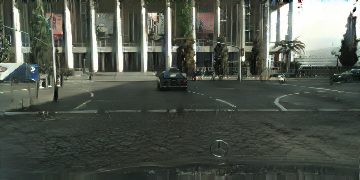
\includegraphics{Section2/train/02003_fake.png}
      & 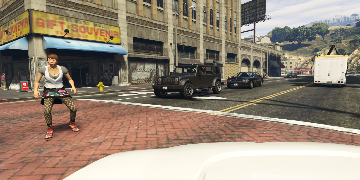
\includegraphics{Section2/train/02788_real.png}
      & 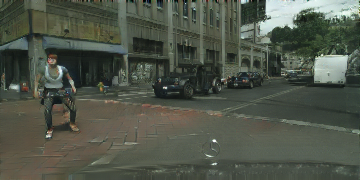
\includegraphics{Section2/train/02788_fake.png} \\
      \rotatebox[origin=c]{90}
      & 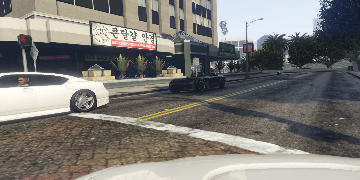
\includegraphics{Section2/train/02015_real.png}
      & 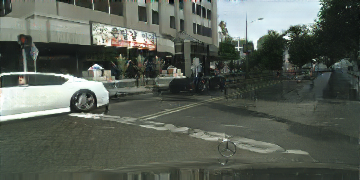
\includegraphics{Section2/train/02015_fake.png}
      & 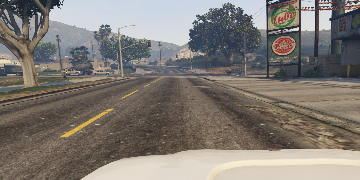
\includegraphics{Section2/train/source_110.png}
      & 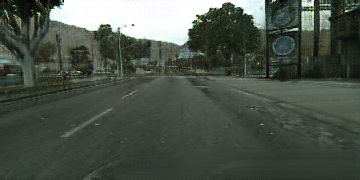
\includegraphics{Section2/train/trans_source_110.png} \\
      \rotatebox[origin=c]{90}
      & 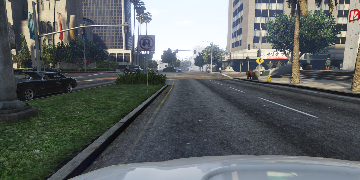
\includegraphics{Section2/train/02013_real.png}
      & 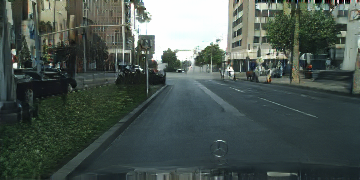
\includegraphics{Section2/train/02013_fake.png}
      & 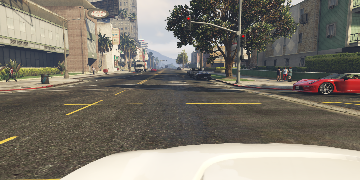
\includegraphics{Section2/train/05990_real.png}
      & 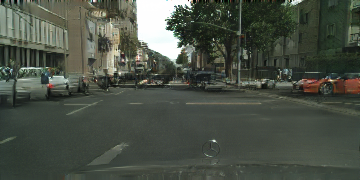
\includegraphics{Section2/train/05990_fake.png} \\
      \rotatebox[origin=c]{90}
      & 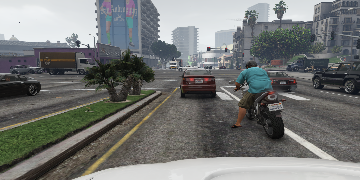
\includegraphics{Section2/train/05890_real.png}
      & 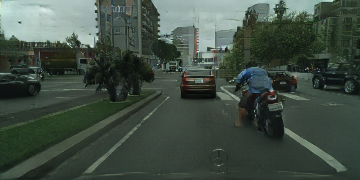
\includegraphics{Section2/train/05890_fake.png}
      & 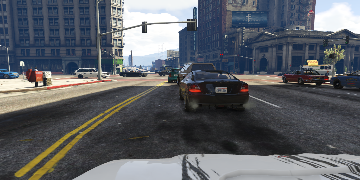
\includegraphics{Section2/train/02382_real.png}
      & 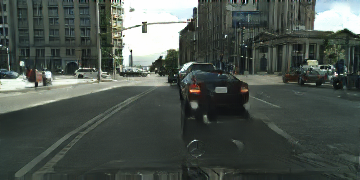
\includegraphics{Section2/train/02382_fake.png} \\
      \rotatebox[origin=c]{90}
      & 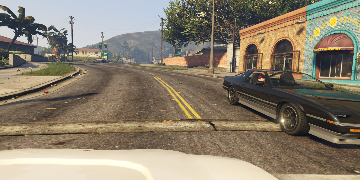
\includegraphics{Section2/train/source_130.png}
      & 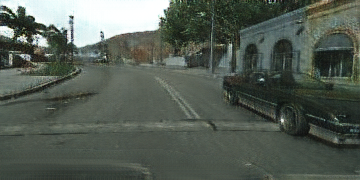
\includegraphics{Section2/train/trans_source_130.png}
      & 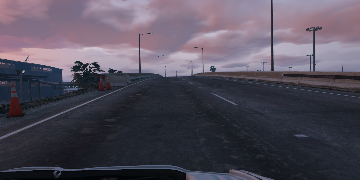
\includegraphics{Section2/train/source_285.png}
      & 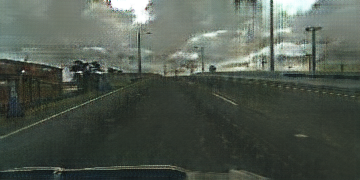
\includegraphics{Section2/train/trans_source_285.png} \\
      \rotatebox[origin=c]{90}
      & 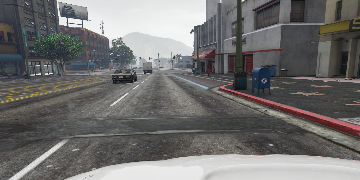
\includegraphics{Section2/train/05834_real.png}
      & 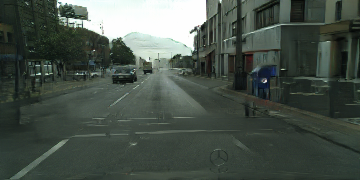
\includegraphics{Section2/train/05834_fake.png}
      & 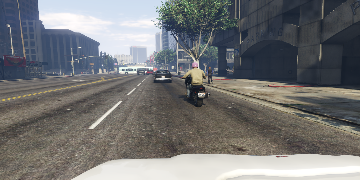
\includegraphics{Section2/train/02050_real.png}
      & 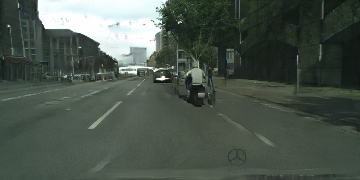
\includegraphics{Section2/train/02050_fake.png} \\
      \rotatebox[origin=c]{90}
      & 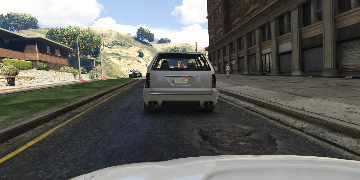
\includegraphics{Section2/train/05802_real.png}
      & 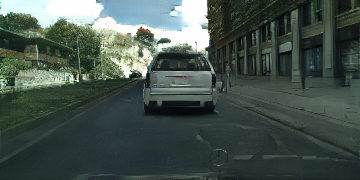
\includegraphics{Section2/train/05802_fake.png}
      & 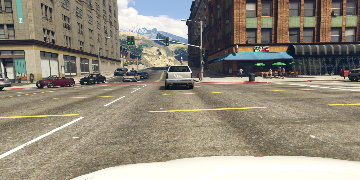
\includegraphics{Section2/train/05796_real.png}
      & 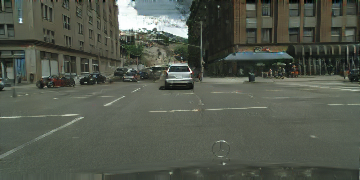
\includegraphics{Section2/train/05796_fake.png} 
    \end{tabularx}
    \caption{Our CycleGAN model evaluation results on training set (left) and testing set (right).}\label{figure:cycgantest}
\end{figure}

Figure~\ref{figure:cycganF} shows CycleGAN's byproduct generator $F$, which converts real-world cityscape into video game style.

\begin{figure}[!ht]
    \setlength\tabcolsep{6pt}
    \adjustboxset{width=\linewidth, valign=c}
    \centering
    \begin{tabularx}{1.0\linewidth}{@{}
        l @{\hspace{2pt}}
        X @{\hspace{4pt}}
        X @{\hspace{4pt}}
        X @{\hspace{4pt}}
        X @{\hspace{4pt}}
      @{}}
      \rotatebox[origin=c]{90}{\footnotesize \textbf{Source}}
      & 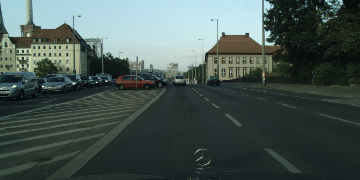
\includegraphics{Section2/train/cityscape2GTA/101_real.png}
      & 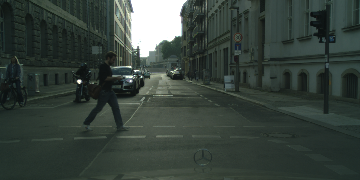
\includegraphics{Section2/train/cityscape2GTA/107_real.png}
      & 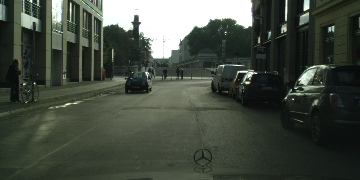
\includegraphics{Section2/train/cityscape2GTA/108_real.png}
      & 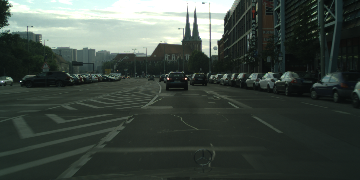
\includegraphics{Section2/train/cityscape2GTA/target_913.png} \\
      \rotatebox[origin=c]{90}{\footnotesize \textbf{Target}}
      & 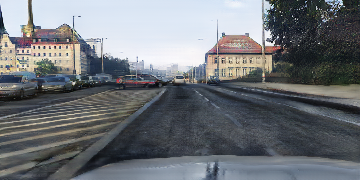
\includegraphics{Section2/train/cityscape2GTA/101_fake.png}
      & 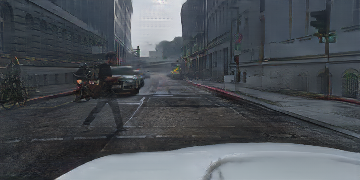
\includegraphics{Section2/train/cityscape2GTA/107_fake.png}
      & 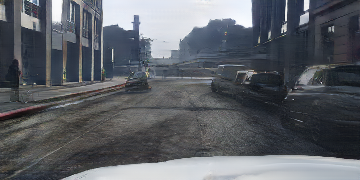
\includegraphics{Section2/train/cityscape2GTA/108_fake.png}
      & 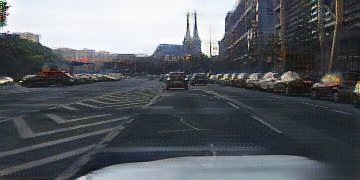
\includegraphics{Section2/train/cityscape2GTA/trans_target_913.png}
    \end{tabularx}
    \caption{The CycleGAN model's byproduct: backward translation results.}\label{figure:cycganF}
\end{figure}

\subsubsection{Major constraints of the CycleGAN}
\paragraph{Wrong recognization of objects.} In Figure~\ref{figure:generate}, we find that CycleGAN has a constraint that recognises the wrong class of objects. For example, it may convert the clouds in the source image into trees in the translated image, or in Figure~\ref{figure:generate} a, it converts the clouds in the source image into buildings in the translated image, and it may also interpret the cloud above the tree in the source image as a portion of the tree, and then generate a huge tree, such as in  Figure~\ref{figure:generate} c. The reason for this phenomenon may be that CycleGAN is better at achieving color and texture changes rather than complex geometric changes, especially clouds and trees with irregular shapes. This limitation was also mentioned by Zhu et al.\ in~\cite{zhu2017unpaired}.

\begin{figure}[!ht]
    \setlength\tabcolsep{6pt}
    \adjustboxset{width=\linewidth, valign=c}
    \centering
    \begin{tabularx}{1.0\linewidth}{@{}
        l @{\hspace{2pt}}
        X @{\hspace{4pt}}
        X @{\hspace{4pt}}
        X @{\hspace{4pt}}
        X @{\hspace{4pt}}
      @{}}
      & \multicolumn{1}{c}{\footnotesize \textbf{(a)}}
      & \multicolumn{1}{c}{\footnotesize \textbf{(b)}}
      & \multicolumn{1}{c}{\footnotesize \textbf{(c)}}
      & \multicolumn{1}{c}{\footnotesize \textbf{(d)}} \\
      \rotatebox[origin=c]{90}{\footnotesize \textbf{Source}}
      & 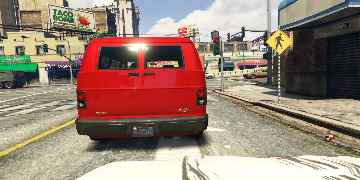
\includegraphics{Section2/test/geometric/02410_real.png}
      & 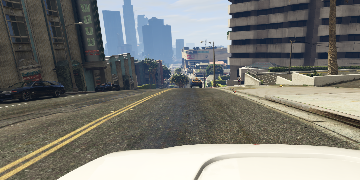
\includegraphics{Section2/test/geometric/02851_real.png}
      & 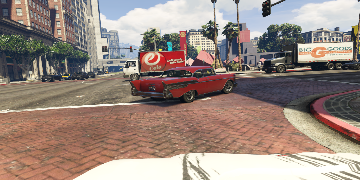
\includegraphics{Section2/test/geometric/02377_real.png}
      & 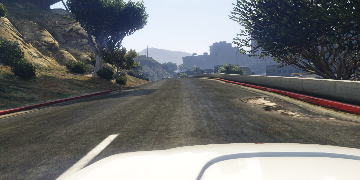
\includegraphics{Section2/test/geometric/03450_real.png} \\
      \rotatebox[origin=c]{90}{\footnotesize \textbf{Target}}
      & 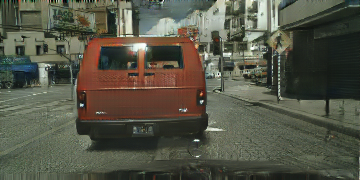
\includegraphics{Section2/test/geometric/02410_fake.png}
      & 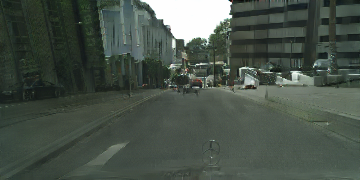
\includegraphics{Section2/test/geometric/02851_fake.png}
      & 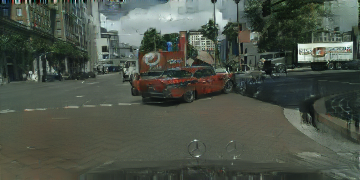
\includegraphics{Section2/test/geometric/02377_fake.png}
      & 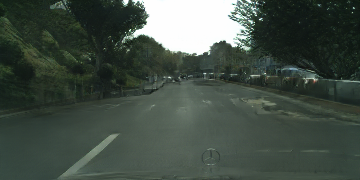
\includegraphics{Section2/test/geometric/03450_fake.png}
    \end{tabularx}
    \caption{Failure cases of the CycleGAN:\@ Wrong recognization of the class of the object.}\label{figure:generate}
\end{figure}

\paragraph{Generation of artifact.} In Figure~\ref{figure:halo} we find that CycleGAN may generate some artifacts that do not exist in the real world, such as in the translated images in examples a, b, and c in Figure~\ref{figure:halo}. A strange dark green patch is generated in the sky. Besides, in example b in Figure~\ref{figure:halo}, in the right part of the image, the image which was originally a sunny sky was translated into an image with a dark cloud artifact. I think the reason for this phenomenon may be the poor performance of the learned discriminators, which may mislead the generator, and thus the image with artifacts may be mistakenly recognized as the correct one when performing reprojection during the training process. As a result, balancing the training speed of discirminators and generators and balancing the adversarial loss and the cycle consistency loss is also a constraint for CycleGAN.\@

\begin{figure}[!htb]
    \setlength\tabcolsep{6pt}
    \adjustboxset{width=\linewidth, valign=c}
    \centering
    \begin{tabularx}{1.0\linewidth}{@{}
        l @{\hspace{2pt}}
        X @{\hspace{4pt}}
        X @{\hspace{4pt}}
        X @{\hspace{4pt}}
        X @{\hspace{4pt}}
      @{}}
      & \multicolumn{1}{c}{\footnotesize \textbf{(a)}}
      & \multicolumn{1}{c}{\footnotesize \textbf{(b)}}
      & \multicolumn{1}{c}{\footnotesize \textbf{(c)}}
      & \multicolumn{1}{c}{\footnotesize \textbf{(d)}} \\
      \rotatebox[origin=c]{90}{\footnotesize \textbf{Source}}
      & 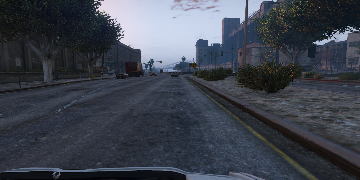
\includegraphics{Section2/test/halo/239_real.png}
      & 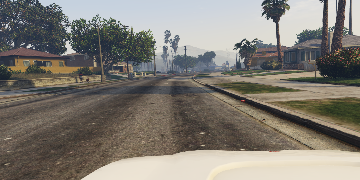
\includegraphics{Section2/test/halo/100_real.png}
      & 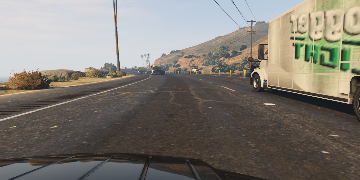
\includegraphics{Section2/test/halo/53_real.png}
      & 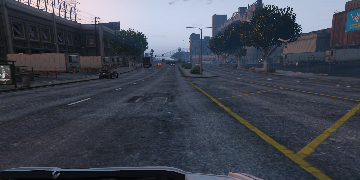
\includegraphics{Section2/test/halo/236_real.png} \\
      \rotatebox[origin=c]{90}{\footnotesize \textbf{Target}}
      & \includegraphics{Section2/test/halo/239_fake.png}
      & \includegraphics{Section2/test/halo/100_fake.png}
      & \includegraphics{Section2/test/halo/53_fake.png}
      & \includegraphics{Section2/test/halo/236_fake.png}
    \end{tabularx}
    \caption{Failure cases of the CycleGAN:\@ Wrong generation of artifact.}\label{figure:halo}
\end{figure}

\paragraph{Perform badly at night and dusk scenes.} In Figure~\ref{figure:unseen}, we observe that CycleGAN performs poorly in night and dusk scenes. In the night scene, it translates the dark sky into the hue that does not exist in real-world cityscapes. In the dusk scene, it translates the orange sky into a sunny sky, failing to accurately capture the temporal information of the original image. The reason for this phenomenon may be the fact that the training set does not contain such images, or there are a few pairs of such training images compared to daytime images. The generalizability of CycleGAN is also very weak compared to other models using the aligned paired training method.

\begin{figure}[!htb]
    \setlength\tabcolsep{6pt}
    \adjustboxset{width=\linewidth, valign=c}
    \centering
    \begin{tabularx}{1.0\linewidth}{@{}
        l @{\hspace{4pt}}
        X @{\hspace{4pt}} 
        X @{\hspace{6pt}} |
        X @{\hspace{4pt}}
        X @{\hspace{4pt}}
      @{}}
      & \multicolumn{1}{c}{\footnotesize \textbf{Source:} night}
      & \multicolumn{1}{c}{\footnotesize \textbf{Target:} night}
      & \multicolumn{1}{c}{\footnotesize \textbf{Source:} dusk}
      & \multicolumn{1}{c}{\footnotesize \textbf{Target:} dusk} \\
      \rotatebox[origin=c]{90}
      & \includegraphics{Section2/test/night/0_real.png}
      & \includegraphics{Section2/test/night/0_fake.png}
      & \includegraphics{Section2/test/night/301_real.png}
      & \includegraphics{Section2/test/night/301_fake.png} \\
      \rotatebox[origin=c]{90}
      & \includegraphics{Section2/test/night/1_real.png}
      & \includegraphics{Section2/test/night/1_fake.png}
      & \includegraphics{Section2/test/night/302_real.png}
      & \includegraphics{Section2/test/night/301_fake.png} \\
      \rotatebox[origin=c]{90}
      & \includegraphics{Section2/test/night/43_real.png}
      & \includegraphics{Section2/test/night/43_fake.png}
      & \includegraphics{Section2/test/night/305_real.png}
      & \includegraphics{Section2/test/night/305_fake.png}
    \end{tabularx}
    \caption{Failure cases of the CycleGAN:\@ Performs poorly in night and dusk scenes.}\label{figure:unseen}
\end{figure}

\paragraph{The fuzzy images and Color distortion.} In the above Figures~\ref{figure:generate},~\ref{figure:halo}, and~\ref{figure:unseen}, we can see that the images generated on the test set have less clarity compared to the source images and there will be some color distortion. The reason for this phenomenon is that we used too few images in the training set or too few epochs. Thus we can conclude that although CycleGAN can learn mappings without paired images, it still needs a lot of data to achieve good results in some cases, especially when the target area changes greatly.

\paragraph{Intrinsic constraints of CycleGAN.} The mapping generated by CycleGAN is a kind of deterministic mapping because cycle consistency enforces $G$, and $F$ to be inverses of each other~\cite{almahairi2018augmented}. When dealing with complex cross-domain datasets, this deterministic mapping causes CycleGAN to learn an arbitrary one-to-one mapping instead of capturing the true, structured conditional distribution more faithfully~\cite{almahairi2018augmented}. At the same time, CycleGAN still does not eliminate the mode collapse problem. It still exists that the generator tends to generate similar or identical outputs while ignoring some subtle differences in the inputs. This may lead to a lack of diversity in the generated results.

\newpage

\section{Feature description and match}


\newpage

% \section{Robust Recovery of Homography}

\newpage

% \section{Image Stitching}



\newpage

% \section{Result discussion}



\newpage

%==== ENDING PART ===

\bibliographystyle{IEEEtran}
\bibliography{Ref/References}

%==== END OF ALL ===
\end{document}
